% options:
% thesis=B bachelor's thesis
% thesis=M master's thesis
% czech thesis in Czech language
% slovak thesis in Slovak language
% english thesis in English language
% hidelinks remove colour boxes around hyperlinks

\documentclass[thesis=M,czech]{FITthesis}[2012/06/26]

\usepackage[utf8]{inputenc} % LaTeX source encoded as UTF-8

\usepackage{graphicx} %graphics files inclusion
% \usepackage{amsmath} %advanced maths
% \usepackage{amssymb} %additional math symbols

\usepackage{dirtree} %directory tree visualisation

% % list of acronyms
% \usepackage[acronym,nonumberlist,toc,numberedsection=autolabel]{glossaries}
% \iflanguage{czech}{\renewcommand*{\acronymname}{Seznam pou{\v z}it{\' y}ch zkratek}}{}
% \makeglossaries

\newcommand{\tg}{\mathop{\mathrm{tg}}} %cesky tangens
\newcommand{\cotg}{\mathop{\mathrm{cotg}}} %cesky cotangens

% % % % % % % % % % % % % % % % % % % % % % % % % % % % % % 
% ODTUD DAL VSE ZMENTE
% % % % % % % % % % % % % % % % % % % % % % % % % % % % % % 

\department{Katedra \ldots (Softwarového inženýrství)}
\title{Distrubuované ukládání a zpracování velkého množství dat - případové studie}
\authorGN{Dominik} %(křestní) jméno (jména) autora
\authorFN{Veselý} %příjmení autora
\authorWithDegrees{Bc. Dominik Veselý} %jméno autora včetně současných akademických titulů
\supervisor{Ing. Michal Valenta, PhD}
\acknowledgements{Doplňte, máte-li komu a za co děkovat. V~opačném případě úplně odstraňte tento příkaz.}
\abstractCS{V~několika větách shrňte obsah a přínos této práce v~češtině. Po přečtení abstraktu by se čtenář měl mít čtenář dost informací pro rozhodnutí, zda chce Vaši práci číst.}
\abstractEN{Sem doplňte ekvivalent abstraktu Vaší práce v~angličtině.}
\placeForDeclarationOfAuthenticity{V~Praze}
\declarationOfAuthenticityOption{4} %volba Prohlášení (číslo 1-6)
\keywordsCS{Nahraďte seznamem klíčových slov v češtině oddělených čárkou.}
\keywordsEN{Nahraďte seznamem klíčových slov v angličtině oddělených čárkou.}

\begin{document}
	
% \newacronym{CVUT}{{\v C}VUT}{{\v C}esk{\' e} vysok{\' e} u{\v c}en{\' i} technick{\' e} v Praze}
% \newacronym{FIT}{FIT}{Fakulta informa{\v c}n{\' i}ch technologi{\' i}}

\begin{introduction}
	%sem napište úvod Vaší práce
\end{introduction}



\chapter{Cíl práce}
Zmínit že práce nikterak nesrovnává klasické a BigData databáze naopak se zabývá open source nástroji od apache

\section{Motivace}
\section{Příprava předmětu}
\section{Rozšíření povědomí}
\section{Praktické zkušenosti}


\chapter{Co jsou to BigData}

Popsat termín BigData není úplně snadné a to z několika důvodů. Předně protože neexistuje žádná přesná definice tohoto pojmu. Tento termín je stejně jako obor, kterého se týká velice dynamický a rychle se mění. V neposlední řadě také proto, že se používá především v marketingové komunikaci jako \uv{Buzzword} za účelem vzbudit zájem čtenáře/posluchače přestože je použit v nesprávném kontextu.

Termín BigData označuje manipulaci s datasety tak velkými, že je nemožné nebo velice obtížné  s nimi manipulovat za pomocí tradičních databází ( převážně relačních) a nástrojů. Pod pojmem manipulace s datasety myslíme:

\begin{itemize}
  \item Sběr
  \item Organizce
  \item Ukládání
 \item Prohledávání
 \item Sdílení
 \item Analýza
 \item Vizualizace
\end{itemize}

Nalezení této hranice, či ji dokonce definovat je komplikovanější problém mimo rozsah této práce a na toto téma bylo napsáno mnoho jiných prací. Jak jsem zmínil v úvodu, práce se nezabývá porovnáním BigData a klasických relačních databází. 

V této kapitole se pokusím obecně přiblížit co to tedy BigData jsou, jak se liší a důvod vzniku tohoto odvětví.


\section{Trend velkých datasetů}
Ja jsem již naznačil, BigData jsou o zpracování velkých DataSetů tento trend upřednostňování velkých datasetů oproti několika menším, které v součtu mají stejný objem a informace začal vzhledem k jednodušímu hledání a objevení i zdánlivě neexistujících korelací, projevení obchodních trendů, či určování určitých jevů v reálném nebo skoro reálném čase. 

\section{3V}
Jak předchozí odstavec naznačil, BigData nejsou pouze o objemu dat jak by se mohlo zdát. Jedná se o komplexnější kategorizaci, kde hrají roli i ostatní charakteristiky, které se v literatuře značí zkratkou 3V odvozenou od počátečních písmen těchto kategorií v anglickém jazyce. 

\begin{figure}[h]
\centering
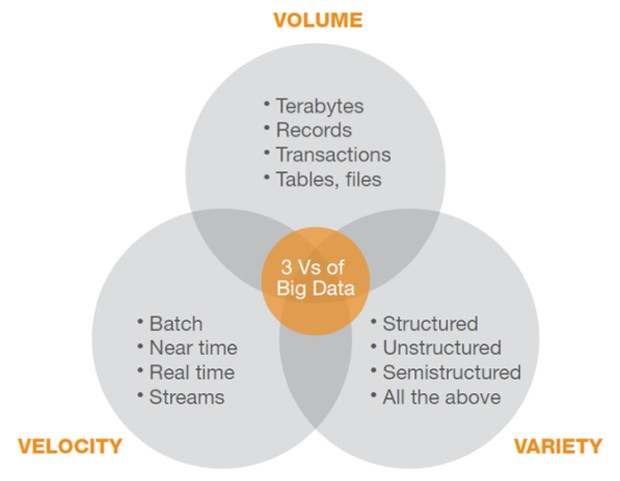
\includegraphics[scale=0.6]{images/3v}
\caption{http://smartdatacollective.com/yellowfin/75616/why-big-data-and-business-intelligence-one-direction}
\label{fig:3v}

\end{figure}

\subsection[3v-volume]{Obsah (Volume)}
Data dnes nejsou pouze v textové podobě, můžeme je uchovávat formou hudby, obrázku či videa. Vzhledem k tomuto faktu čelíme obrovskému exponenciálnímu nárůstu dat a není vyjimečné aby enterprise systémy uchovávaly Terabyty nebo Petabyty dat. Data tedy tvoří množství informaci, které jsou dost často vyhodnocovány z různých úhlů a následně uloženy a znovu vyhodnocovány a přestože původní data zůstala nezměněna, díky reevaluaci nám data rostou ohromným způsobem a takto může být na objem nahlíženo jako na jednu z charakteristik.

\subsection{Rychlost (Velocity)}
Na rychlost můžeme nahlížet hned ze dvou pohledů. Prvním jak rychle nám data přibývají a jak aktuální pro nás jsou. Například historie vývoje měnového kurzu je informace, jejíž včerejší hodnota je naprosto nevypovýdající a mění se i každou minutu. Změnila se i rychlost jakou noviny a televizní stanice získávají informace skrze sociální sítě. Data tedy rostou rychle a aktuálnost informací se rapidně zkrátila. Druhý pohled na tuto charakteristiku značí jak rychle data potřebujeme zpracovávat. Jsou informace které k nám proudí velice často například každou minutu ale jejich vyhodnocení dává smysl jednou za 24 hodin. Ale jsou také data které potřebujeme zpracovávat v reálném čase rovnou jak knám proudí. Například data z meteorologické stanice. 
Rychlost s jakou jsou data dnes potřeba zpracovat se mnohonásobně zmenšila a tedy nejen objem dat ale i rychlost zpracování reprezentuje BigData.

\subsection{Různorodost (Variety)}
Jak je z Obrázku ~\ref{fig:3v} patrné různorodost dat znamená jejich strukturovanost/nestrukturovanost. Jak bylo zmíněno, data mohou mít mnoho podob. Ale i data ve stejné podobě například textové, mohou být jinak strukturovány a tomuto faktu je potřeba se přizpůsobit a uchovávat a zpracovávat data v jiných formátech. Tato různorodost a adaptabilita je tedy poslední charakteristikou BigData

\section{BigData zjednodušeně}
Předcházející řády by měli sloužit jako shrnutí a lehký úvod do problematiky BigData. Dalo by se také říci, že BigData není jen o velkém množství dat ale je to celý koncept uchovávání a možnosti nových náhledů stávající data a také návod jak zachytit a zpracovat budoucí data. Další odstavce budou věnovány historii tohoto konceptu, ale také nejtypičtějších odvětví, kde se vyskytuje. 

\section{Historie}

Již od počátků počítačové éry byla data potřeba analyzovat. \cite{history} Avšak s rychle rostoucí dostupností technologií a jejich obecnému přijetí ve společnosti se posouvala hranice této potřeby od vladních organizací až po současnost, kdy obrovské množství informací a jejích analýzu potřebují i malé podníky

\subsection{30. a 40. léta}
V této době se použivali první počítačové simulace především ve válečném odvětví kdy například vědci z Manhattan projektu pomocí počítačových simulací, simulovali dopad a efekt jaderné bomby

\subsection{50. a 60. léta}
V tomto období se počítače a celkově zpracování a anlýza dat rozšířila o velké korporace a výzkumné laboratoře. Počítač ENIAC generoval první modely předpovědi počasí. Analytici vyřešili první problém nejkratší cesty a mnoho dalších viz. \cite{history}

\subsection{70. až 90. léta}
V této době se analytická činnost rozšířila o středně velké podniky a technologické startupy a objevují se dnes známe případy užití. První predikční model na pokles a růst akcií. První komerční nástroj pro modelově řízené rozhodování a hlavně Společnosti jako Ebay a Amazon startují svou činnost, bitva o perzonalizaci online nákupů právě začala! Google implementuje první vyhledávací algoritmus, který zvyšuje relevanci výsledků.

\subsection{2000 až součanost}
V tomto období se analytika a rozšířila až na oblast malých podniku a analytických expertů jednotlivců. Analytika začíná mít obrovský dopad na život. Dynamické změny cen zboží, doporučení produktů, hudby a filmů nebo řízení dopravy. analýza a procesování přirozeného jazyka z novin, emailů nebo sociálních sítí. Příchod Big Data, vzhledem k levné dostupnosti výpočetního výkonu a rychlosti zpracování dat, se stává tato možnost dostupnout téměř pro kohokoliv.

\subsection{Budoucnost}
V budoucnu se předpokládá, že analytická činnost se rozšíří do každodenního užití i pro jednotlivce a bude tak řídit jejich rozhodnutí. V běžném životě se také předpokládá, že analýza dat přinese například. Predikce v policejní sféře a boji proti zločinu, výzkum ve zdravotnictví nebo kompletně personalizovaná zákaznická interakce i pro malé podniky a řetězce.

\section{Nástup sociálních sítí}
Big Data zažila obrovský nástup také díky příchodu a masivnímu rozšíření sociálních sítí a to hned ze dvou důvodů. Prvním důvodem je, že nástup sociálních sítí přilálakal tisíce výzkumníků, kteří začali sbírat data z Facebooku a Twitteru a hledali různá spojeni mezi zprávami a účty z nich pak vyvozovali závěry ohledně těchto sociálních sítí. Další možností k čemu vytěžená data použivali bylo k vytváření tzv. sociálních grafů. Historicky sbírali antropologové a sociologové data o lidských vztazích skrze dotazníky, rozhovory, pozorování a experimenty. dolováním dat ze sociálních sítí, kde lidé sdílejí mnoho detailů ze svých životů se jim otevřel nový kanál, kde mají všechny tyto informace jednouše k dostání a stačí je pouze analyzovat.

BigData podle vědců představájí 2 druhy sociálních sítí: \uv{Artikulované sítě} a \uv{Behaviorální sítě}. První kategorie znázorňuje sítě, kde uživatelé zadávají své přátelé a konexe skrze technické mechanismy jako například: telefonní seznamy, emaily, seznamy přítel z jiných sití atd. Druhou kategorií jsou sítě odvozené od komunikačních vzorců. Do této skupiny spadají uživatelé, kteří si píšou zprávy nebo jsou označení na společných fotkák. Obě ty to skupiny mají pro výzkumníky velký význam přestože jím nepřikládají takovou váhu jako reálným osobním vztahům. \cite{social}

Druhým důležitýn aspektem, proč jsou sociální sítě pro Big Data důležité, je fakt, že tyto sítě samy potřebují někde svá data uchovávat a zpracovávat a proto tedy technologické týmy těchto služeb vytvářejí velké \% kolaborátorů v BigData projektech, či dokonce vytvářejí a následně uvolňují svoje technologie a nástroje k užití pro širokou veřejnost. Pro komunitu jsou důležité i přednášky a prezentované poznatky od těchto datových gigantů, kteří prozkoumavájí a prolamují lidstvu dosud známe bariéry a umožňují tím využívání technologických pokroků i jiným subjektům. 

Sociální sítě samozřejmě nejsou jediným průkopníkem na poli BigData, internetový giganti jako Google, Amazon a Yahoo také přispívají stejným dílem, na sociálních sítích je však zajímavé to, že jejich data jdou do jisté míry jednoduše dolovat a tak vzniklo mnoho spolčeností, které se začali analýzou a sběrem zabývat a způsobili tím popularizaci spojení BigData se sociálními sítěmi. 


\section{Odvětví}

Jak bylo v předchozí sekci zmíněno, v dnešní době můžeme na BigData narazit kdekoliv a v jakémkoliv odvětví. Zde bych chtěl poukázat na široké spektrum využití napříč různými činostmi, kterým se lidstvo zaobírá.\cite{sektory}

\subsection{Maloobchod}
Péče o zákazníka a samozřejmě i zvýšení zisku jsou hlavními motivy pro zpracovávání a analýzu dat. Ná základě chování uživatelů (aktivita na webu, zákaznická karta, anonymni zákazníci) předpovídat chování zákazníka v každém stádiu nákupu. Lze spojit i s podnikovými daty a hledat korelace pomocí Map Reduce mechanizmů. Největším průkopníkem spojení BigData a maloobchodu je bezesporu řetězec Tesco se svou věrnostní kartou ClubCard. Kde na základě uživatelovi nákupní historie, sestavují žebříček produktů k doporučení, či dokonce odhadují dané obdboí těhotenství svých zákaznic.\cite{tesco}

\subsection{Věda a výzkum}

Není žádným překvapením, že ve vědě a výzkumu se využívají Big Data na uchovávání výsledků z měření, či hledání korelací v naměřených výsledcích. Například držitel Nobelovy ceny Peter Higgs používal NoSQL databázový systém Cassandra na zpracování svých dat, díky nímž prokázal existenci tzv. Higgsova Bosonu \cite{higgs}

\subsection{Meteorologie}
Díky sběru a vyhodnocování dat z meteorologických stanic se podařilo vytvořit mnohem spolehlivější a přesnější modely pro předpovědi počasí a to jak dlouhodobých, tak krátkodobých. 

\subsection{Finance}
Zde je způsobů užití hned několik, například již výše zmíněné doporučování produktů, dle historie transakcí a sběru  osobních dat, banky a jiné finanční instituce navrhují vhodné finanční produkty jako například hypotéky. Druhým mnohem zajímavějším případem využití je detekce podvodů, kde jsou banky na základě analýzy všech transakcí hledat vzory podvodných chování a vyhodnotit určité transakce jako podezřelé a tím tak chránit své klienty nebo sami sebe.

\subsection{Webová optimalizace}
Na základě ukládání a následného zpracování veškěrého chování uživatele na stránce, mohou firmy optimalizovat webové stránky a jejich obsah, či ho případně restrukturalizovat. Po vyhodnocení chování konkrétních uživatelů jde obsah stránky automaticky personalisovat a podsouvat uživatelům pro ně zajímavé věci, aniž by se k nim museli proklikávat.

\subsection{BioInformatika}
V Bioinformatice se BigData využívají například k mapování genomů nebo sekvenční analýze. Tyto informace pomáhají k lepšímu pochopení DNA a také prevence genetických poruch a vrozených nemocí, či usnadnění jejich léčby. \cite{industries} 

\section{Dnešní možnosti}
V dnešní době existují v podstatě 3 možnosti jak začít s BigData. 

\subsection{Specilizované firmy a hotová řešení}
Na internetu nalezneme několik firem zabývajících se analýzou vašich dat, kde veškerá analýza a vizualizace probíhá v softwaru třetí strany. Mezi nejznámější patří společnost Good Data ycite{gooddata}. Tyto firmy se však specializují na zpracování firemních dat a vizualizaci v jejich vlastních BI nástrojích.

\subsection{Hotová enterprise řešení}
Další možností je vybrat něaké komplexní řešení od firem zabývajících se platformou BigData, která vám dodá software pro ukládání, analýzu a vizualizaci vašich dat. Programování komponent, či konfigurace je v režii zákazníka a tyto firmy poskytují licence, školení a technickou podporu. Tuto možnost postkytuje například IBM.

\subsection{Open Source a řešení z něj vycházející} 
Poslední možností je použití Open Source nástrojů, které umožní ukládat, analyzovat a vizualizovat data. Toto je cesta, kterou jsem vybral v této práci a budu se mu až do konce této práce věnovat. Drobnou nadstabou těchto řešení jsou firmy poskytující komerční balíčky těchto opensource řešení. Jedná se o velice populární přístup, pokud je potřeba zkombinovat několik nástrojů dohromady je jejich konfigurace velice obtížná a tyto komerční balíčky jsou již nakonfigurovaná hotová řešení většinou i s drobnou nadstavbou která umožnujě některé procesy a činnosti. 


%mozna jen podsekce bigdata%
\chapter{BigData techniky}
Abychom mohli hovořit o konkrétních technologicích, musíme nejdříve definovat základní stavební technologické kameny, o které se BigData opírají. Jedná se o technologie a paradigmata vyvinutá technologickými giganty, kteří jako první naráželi na technologické hranice a posouvali je dál a tak se postupně rodily tyto technologie a paradigmata. Jejich pořadí se odvýjí od logické posloupnosti tak, jak spolu souvisí a navazují na sebe.    

\section{Distribuované systémy}
Distribuované systémy, jsou tématem, které zasahuje samozřejmě mnohem dále, než jen do kategorie big data. Pro zjednodušení následujících řádků, zavedeme následující rozdělení. Distribuované systémy rozdělíme na systémy s distribuovaným výpočetním výkonem, systémy s distribuovaným úložištěm a nebo kombinace obojího. 

Distribuovaný výpočetní výkon, je takový systém, kde se výpočet jedné úlohy rozloží na více počítačů. Paralelní výpočety jsou známé z oblasti informačních technologií, již mnoho let a používají se nejčastěji k vědeckým výpočtům, paralelní kompilaci zdrojových kódů a nebo k jiným operacím, které by na jednom počítači trvaly příliš dlouho. 

Distribuované úložistě je jednoduše představitelné a důvodů mít data na více místěch je hned několik.
\begin{itemize}
\item Záloha - i ze sféry osobních počítačů známé trend kde máme data zálohovaná na více fyzických zařízeních, abychom předešli jejich ztrátě, v případě technické poruchy na daném zařízení. 

\item Nedostatek kapacity - Ze sféry osobních počítačů známe, že uživatelé, méně potřebné soubory ukládají na externí periferie, protože kapacita disků v osobních počítačích je zpravidla kolem pár TB.

\item Dostupnost - Pokud chce uživatel mít přístup k jednomu souboru z domácího i pracovního počítače, musí soubor mít fyzicky na těchto dvou počítačích, nebo využít nějaký software na sdílení souborů. 

\end{itemize}

Kombinovaný přístup je zřejmy a tedy, že se používá jak výpočetní výkon jednotlivých počítačů v systému, tak jejich úložný prostor. 

Big Data využívá všechny tyto přístupy, je zřejmé že obrovské množství dat, o kterém jsme mluvili v úvodu se lépe zpracovává na více počítačích. Stejně tak je logické, že pokud budeme bavit o množství dat, tak velké množství dat, uložíme na více počítačů, stejně tak pokud data chceme zálohovat. 

Ne vždy však využíváme kombinovaný přístup, je totiž velmi časté, že si firmy staví obrovské počítačové farmy, které slouží pouze jako datové sklady a datová centra. Vždy záleží na konkrétní situaci a způsobu využití. 


\section{CAP Theorem}
V roce 2000 při nástupu distribuovaných systémů vydal vědec Eric Brewer článek, popisucjíí tzv. CAP Theorem \cite{cap}, který se distribuovaných systémů přímo týká. Teorém říká, že distribuované systémy mají tyto 3 hlavní vlastnosti. 

\begin{itemize}
\item Konzistence (Consistency) - Vlastnost, která určuje, zda pro každý požadavek, vratí server správný výsledek. to znamena že odpověd je adekvátní vůči specifikaci požadované služby. Přesný význam konzistence se odvýjí od typu služby. V případě dat ji definujeme tak, že každý server má aktuální a stejná data.

\item Dostupnost (Availability) - Vlastnost která říka, že každý požadavek dostane odpověd. Rychlejší odpověd, je preferovanější oproti pomalejší, ale v kontextu teorému je důležité, že odpověd dorazí. V praxi však znamená, že velice opožděná odpověd je stejně spatná jako žádná odpověd a můžeme tuto vlastnost zjednodušit, že systém vždy musí být dostupný.

\item Tolerance výpadku (Partiotion tolerance) - Tato vlastnost jako jediná určuje chování podpůrného systému na kterém služba běží, namísto popisu chování služby samotné. Tato vlastnost říká, jestli během výpadku nějaké části systému, je systém schopný pokračovat a dále fungovat.

\end{itemize}


Brewer popisuje, že každý distribuovaný systém může splňovat nejvýše 2 z těchto 3 vlastností.

\subsection{CAP Theorem v roce 2012}
V roce 2012 napsal Brewer další článek \cite{cap2}, ve kterém popisuje stav jeho theorému po 12 letech. Vysvětluje, že již od začátku bylo označení \uv{pouze 2 ze 3} zavádějící a vágní, protože spoustu věcí příliš zjednodušovalo. Například u systému s velkou granularitou,  se mezi volbou C a A rozhoduje na několika úrovních a všechny vlastnosti mají spíše hodnoty v čase, než binární a také, že záleží na stavbě systému a jeho drobných nuancích. Také ale píše, že v důsledku theorém splnil svůj účel a otevřel tak systémévým návrhárům oči pri navrhování distribuovaných systémů a donutil je zamyslet se nad vyhodami a nevýhodami jednotlivých vlastnotí systému. 

V témže roce vyšel další zajímavý článek popisující aktuální stav CAP theorému \cite{cap3}. Popisuje převážně vztah
systémů k volbám CAP vlastnostní. 

\subsubsection{Nejlepší možná dostupnost}
Nejčastejší výběr je garantovaná konzistence s maximální možnou dostupností, pro většinu systémů je toto přirozenou volbou. Tedy, že za každou cenu, server vrací správnou odpověd a snaží se poté optimalizovat co největší dostupnost a nejrylechjší možnou odpověd vzhledem k síťovým podmínkám. Tento přístup dává největší smysl pokud jsou počítače ve stejném datacentru a běží na nich stejná služba. Typickým zástupcem je  \uv{lock service} a služba spravující metada pro nějaký distribuovaný systém s nízkou granularitou.

\subsubsection{Nejlepší možná konzistence} 
Druhou nejčastější skupinou jsou systémy, pro které je ztráta dostupnosti nemyslitelná a tudíž garantují dostupnost a snaží se o co nejvyšší úroveň konzistence. Tento postup nejlépe vyhovuje v případech kdy máme počítače distribuované napříč několika datacentry, v tomto případě může totiž dostupnost rapidně klesat s jakoukoliv chybou a proto je potřeba ji garantovat. V těchto případech tedy designéři obětují konzistenci, aby mohli garantovat dostatečně rychlou odpověd, přestože ta nemusí být vždy zcela správná. Ideálním příkladem jsou webové cache a obrázkové servery.

\subsubsection{Segmentovaná konzistence a dostupnost}
toto je nejzajímavější možnost a pro tuto práci je také nejdůležitější. Existují systémy, které nemají jednotné požadavky pro všechny aspekty služby. Některé vyžadují silnou konzistenci a některé vysokou dostupnost. Pro dodžení CAP theoremu se  jako nejpřirozenější možnost jeví rozdělit systém na několik jednotlivých komponent, které budou specificky nastaveny. tím tedy celý systém nezaručuje ani konzistenci, ani dostupnost, ale každá část systému postkytuje opravdu vlastnosti, které potřebuje. Segmentace může probíhat na několika možných úrovních. 

\begin{itemize}
\item \textbf{Rozdělení podle dat} - jiná data mohou vyžadovat jinou úroveň dostupnosti a konzistence.
\item \textbf{Rozdělení podle operací} - Operace pro zápis mohou mít jiné požadavky na konzistenci a dostupnost, než operace pro čtení.
\item \textbf{Rozdělení podle funkcí} - Některé služby mohou být rozděleny na podslužby a tedy pro každou takovouto službu můžeme mít vlastní úroveň konzistence a dostupnosti. 
\item \textbf{Rozdělení podle uživatelů} - Jedná se o rozdělení závislé převážně na geografické poloze uživatele, služba bude pro uživatele, který se nachází blízko může zaručit vysokou dostupnost a zároveň v rámci jeho blízkého data centra udržovat i konzistenci. 
\item \textbf{Rozdělení podle hierarchie} - Jedná se o systém ve kterém se na určitých úrovních kombinují výše popsané rozdělení.
 
\end{itemize}
\section{Distribuovaný file systém}

V předchozích sekcích jsme rozebrali distribuované systémy a jejich omezení. Zmínili jsme také, nutnost sdílet velké množství dat napříč několika počítači, které můžou být napříč různými datacentry. Tuto potřebu, tedy mít distribuovaný filesystém, měl i jeden z největších technologických gigantů, firma Google. V roce 2004, se Google rozhodl o jejich řešení podělit a vydal detailní článek \cite{gfs} popisující kompletní funkčnost a detaily celé infrasntruktury. Vysvětlení funkčnosti a  architektury je nad rámec této práce a navíc je vše dobře popsané v článku samotném, důelžité je však zmínit, že tento systém se stal inspirací a nastolil trend v tom, jak podobné systémy dnes vypadají a jaké mají vlastnosti. Na základě tohoto článku vznikl například opensource klon MooseFS.

\begin{figure}[h]
\centering
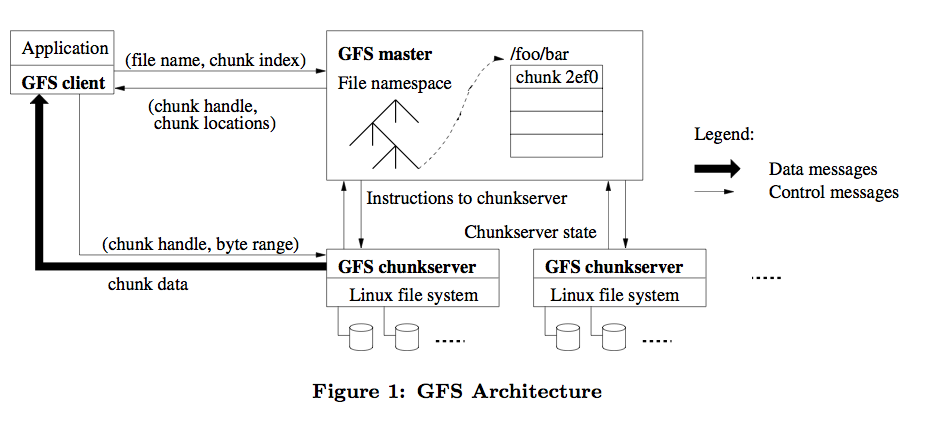
\includegraphics[scale=0.5]{images/gfs}
\caption{Architektura Google File System \cite{gfs}}
\label{fig:3v}
\end{figure}

\section{BigTable}
Jedná se o systém na uchovávání dat spoledčnosti Google, který je postavený nad Google File Systémem a jinými technologiemi společnosti Google. Jedná se o proprietární software, který není kdispozici mimo firmu Google, kromě možnost využívat tento sw jako část služby Google App Engine.  V roce 2006 opět google zveřejnil článek o BigTable \cite{bigtable}, avšak nyní s mnohem méně detaily, nežli u svého článku o GFS \cite{gfs}, kvůli obavám o přesné zkopírování jako u zmíněného systému. V době vydání článku bigtable obsluhoval více než 60 služeb firmy Google a škáloval několik Petabytů dat na několika tisici počítačích. BigTable umožňuje využívání MapReduce frameworku. Jedná se o první implementaci mnoho sloupcové, distribuované, multidimenzionální perzistentní seřazené mapy.  Google opět udal trend jakým se podobné systémy začali ubírat. Datový model BigTable v budoucnu inspiroval i tvůrce Apache Cassandra, která je hlavním tématem této práce a proto detaily ohledně datového modelu prozatím přeskočíme.

\section{MapReduce}
Je programovací model a framework prvně představený společností Google \cite{mapreduce} na zpracování velkého datasetu. Uživatel specifikuje mapovací funkci, která zpracuje páry (klíč, hodnota) a vygeneruje přechodné páry (klíč hodnota), které jsou pak předané redukovací funkci, která sloučí všechny mezi-hodnoty se stejným mezi-klíčem. Mnoho příkladů z reálného světa, lze převézt do tohoto paradigmatu. Výhodou těchto funkcionálně napsaných programů je, že jsou automaticky velice paralelizovatelné. Systém se stará o detaily distribuce dat a rozhození jednotlivých uloh na jednotlivé počítače a obsluhuje chyby a neočekávané stavy. toto umožňuje programátorům i s velice malou znalostí paralelního programování napsat vysoce paralelní a efektivní programy. 

Toto paradigma se stalo v nejdůležitějším stavebním kamenem pro zpracovavání BigData. Díky tomuto mechanizmu jsme schopni zpracovávat Terabyty dat rychle a efektivně a vypočítaný výsledek znovu uložit do databáze. Veškeré postupy zpracování BigData jsou přímo, či nepřímo založené na MapReduce. 

\begin{figure}[!h]
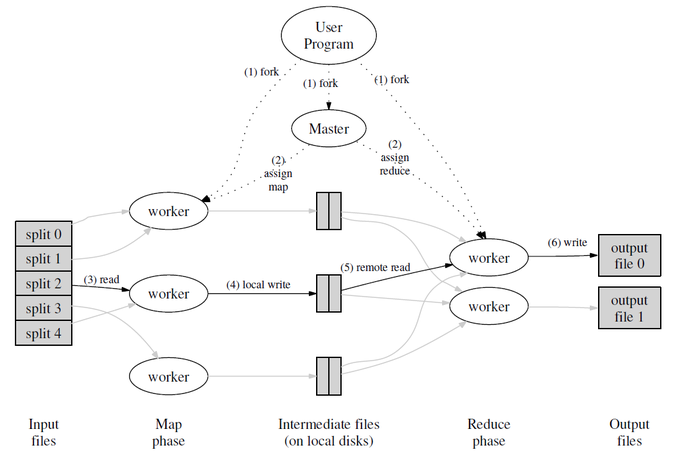
\includegraphics[scale=0.6]{images/mapreduce}
\caption{MapReduce schéma \cite{mapreduce}}
\label{fig:mapreduce}
\end{figure}

\newpage

\section{NoSQL}
Se zkratkou SQL se můžeme u relačních databázových systémů. Zkratka NoSQL neznamená pravý opak, písmena \uv{No} znamenají \uv{Not Only}, tedy ne pouze. Jedná se o databázový koncept, který se vyskytuje u nerelačních databází. V tomto konceptu datové úložiště i zpraování dat používají jiné prostředky, než běžné tabulkové schéma relační databáze. Výhody tohoto konceptu jsou jednoduchá desihn a horizontální i vertikální škálovatelnost. NoSQL databáze často podporují také podmnožinu jazyka SQL a většinou se jedná o jednoduché funkce jako vkládání a velice jednoduché výběry. Některé NoSQL databáze mají i velice odlišný ukládací model, například (stromový, grafový) tím padem je složitost  pro různé operace odlišná. Nejčastější podobu má NoSQL databáze formou klíč hodnota, čili mapa. Podle dosavadních informací lze říci, že Google BigTable je tedy NoSQL databáze. Mezi charakteristiky NoSQL databází můžeme zahrnout

\begin{itemize}
\item \textbf{Datový a dotazovací model} - jak již bylo řečeno NoSQL databáze se liší způsobem udržování dat a  dotazováním nad nimi
\item \textbf{Perzistence} - Ne všechny NoSQL datbáze ukládají svá data na disk, některé databáze běží pouze v operační paměti.
\item \textbf{Rozhraní} - Některé databáze komunikují skrze REST rozhraní a některé pomocí binárních protokolů 
\item \textbf{BASE} - Tak jako relační databáze využívají vlastnosti ACID (Atomic Consistent Isolation Durability) tak v NoSQL je ekvivalentem BASE (Basically Available, Soft state, Eventual consistency) kde každá NoSQL databáze garantuje jednotlivé vlastnosti různými mechanizmy a nastaveními nebo jsou již od základu navržené s danými vlastnostmi.   
\end{itemize}


NoSQL databáze jsou dalším základním stavebním kamenem BigData. NoSQL databáze jsou často kompatibilní s MapReduce konceptem, čímž tvoří ideální dvojici pro uchovávání a zpracování velkého množství dat. 



\chapter{BigData Platforma Apache}
\section{Hadoop}
\section{HBase}
\section{Cassandra}
\section{Hive}
\section{Pig}
\section{SolR}


\chapter{Vhodné případy užití}
\section{Analýza Access logů}
\section{Image Servery}


\chapter{Implementace některých případu užití}
\section{Testovací prostředí}
\section{Implementace Access Log analyzéru}

\begin{conclusion}
	%sem napište závěr Vaší práce
\end{conclusion}

\nocite{*}
\bibliographystyle{csn690}
\bibliography{mybibliographyfile}

\appendix

\chapter{Seznam použitých zkratek}
% \printglossaries
\begin{description}
	\item[GUI] Graphical user interface
	\item[XML] Extensible markup language
\end{description}

\chapter{Obsah přiloženého CD}

%upravte podle skutecnosti

\begin{figure}
	\dirtree{%
		.1 readme.txt\DTcomment{stručný popis obsahu CD}.
		.1 exe\DTcomment{adresář se spustitelnou formou implementace}.
		.1 src.
		.2 impl\DTcomment{zdrojové kódy implementace}.
		.2 thesis\DTcomment{zdrojová forma práce ve formátu \LaTeX{}}.
		.1 text\DTcomment{text práce}.
		.2 thesis.pdf\DTcomment{text práce ve formátu PDF}.
		.2 thesis.ps\DTcomment{text práce ve formátu PS}.
	}
\end{figure}

\end{document}
